\chapter{Comparações}

    \par Este capítulo apresenta uma comparação entre a API REST original desenvolvida em MVC e sua versão refatorada com Arquitetura Limpa. A análise destaca as principais mudanças na estrutura do projeto e no fluxo das requisições, estabelecendo uma base para a compreensão dos resultados apresentados nas seções seguintes. Dessa forma, busca-se proporcionar uma visão geral da refatoração, evidenciando os impactos e aspectos que devem ser considerados na adoção da Arquitetura Limpa, os quais serão discutidos posteriormente neste trabalho.
    
    \section{Comparação Estrutural}
        \par Para apresentar a materialização do modelo conceitual proposto por \cite{livro:martin:cleanarch}, a Tabela \ref{tab:mapeamento_clean_arch} apresenta o mapeamento direto entre cada componente teórico e a sua respectiva representação no projeto, utilizando o caso de uso de criação de um novo contato como exemplo.
        
        \begin{table}[H]
            \caption{Mapeamento dos Componentes}
            \label{tab:mapeamento_clean_arch}
            \begin{tabularx}{\linewidth}{|l|X|} % Adicionados os "|" para as linhas verticais
                \toprule
                % A linha do cabeçalho foi envolvida por {\small ...} para diminuir a fonte
                {\small \textbf{Componente no Cenário Típico (Martin, 2019)}} & {\small \textbf{Classe/Artefato Implementado no Projeto}} \\
                \midrule
                Controller                  & \texttt{CreateContactController.php} \\
                Input Boundary (Interface)  & \texttt{CreateContactInputBoundary.php} \\
                Use Case Interactor         & \texttt{CreateContactInteractor.php} \\
                Input Data                  & \texttt{CreateContactRequestModel.php} \\
                Entities                    & \texttt{Contact.php} (Entidade Pura) \\
                Data Access Interface       & \texttt{ContactRepositoryInterface.php} \\
                Data Access (Implementação) & \texttt{ContactRepository.php} \\
                Database                    & MySQL (Serviço Docker) \\
                Output Boundary (Interface) & \texttt{CreateContactOutputBoundary.php} \\
                Presenter                   & \texttt{CreateContactApiPresenter.php} \\
                Output Data                 & \texttt{CreateContactResponseModel.php} \\
                View Model                  & \texttt{ContactViewModel.php} \\
                View                        & Resposta JSON \\
                \bottomrule
            \end{tabularx}
        \end{table}
       
        \par Essa tradução da teoria para a prática se inicia com o Controller, representado pela classe \texttt{CreateContactController.php}, que transforma a requisição em um Input Data, implementado como o DTO \texttt{CreateContactRequestModel.php}. Este objeto é então passado para o Use Case Interactor (\texttt{CreateContactInteractor.php}) através da Input Boundary, o contrato definido pela interface \texttt{CreateContactInputBoundary.php}. No núcleo da aplicação, o Interactor orquestra as Entities, materializadas pela classe pura \texttt{Contact.php}. 
        
        \par A persistência dos dados é abstraída pela Data Access Interface (\texttt{ContactRepositoryInterface.php}), cuja implementação concreta é o \texttt{ContactRepository.php}, que por sua vez interage com o Database (MySQL). Ao final do fluxo, o Interactor produz o Output Data (\texttt{CreateContactResponseModel.php}) e o entrega ao Presenter (\texttt{CreateContactApiPresenter.php}) através da Output Boundary (\texttt{CreateContactOutputBoundary.php}). Por fim, o Presenter formata esses dados em um View Model (\texttt{ContactViewModel.php}), que serve de base para a View, representada pela Resposta JSON final.

        \par Aprsentados os componentes resultantes da aplicação da Arquitetura Limpa, pode-se realizar uma comparação entre a arquitetura MVC e a Arquitetura Limpa no contexto desse TCC, apresentando as diferenças entre a abordagem inicial, centrada no framework, e a abordagem final, centrada no domínio de negócio. 
        
        \par A primeira mudança perceptível está na organização dos diretórios. A estrutura MVC original agrupa os arquivos por seu tipo técnico (Models, Controllers), enquanto a nova estrutura os organiza por camadas e funcionalidades, refletindo o conceito de "Arquitetura Gritante".
        
        \par Nesse sentido, nota-se que a API base, seguindo o padrão Laravel, possuía uma estrutura enxuta, com a lógica de negócio, acesso a dados e controle de requisições concentradas principalmente nos diretórios \texttt{app/Http/Controllers} e \texttt{app/Models}, conforme consta na Figura~\ref{fig:estrutura-original} onde é apresentada a estrutura do diretório \texttt{app} da API REST base. 

        \begin{figure}[h!]
            \caption{Estrutura do diretório app antes da refatoração.}
            \label{fig:estrutura-original}
            \dirtree{%
            .1 app/.
            .2 Http/.
            .3 Controllers/.
            .4 ContactController.php.
            .4 Controller.php.
            .2 Models/.
            .3 Contact.php.
            .3 User.php.
            .2 Providers.
            .3 AppServiceProvider.php.
            }
        \end{figure}

        \par Já após a refatoração, a estrutura de diretórios passou a refletir as camadas da Arquitetura Limpa. As regras de negócio agora residem em \texttt{app/Entities} e \texttt{app/UseCases}, completamente isoladas do framework. Os componentes que interagem com o mundo externo, como Controllers e Repositories, foram movidos para \texttt{app/InterfaceAdapters}, e os detalhes de implementação específicos do Laravel, como os Models do Eloquent, para \texttt{app/FrameworksAndDrivers}. A Figura \ref{fig:estrutura-depois} demonstra a organização final do diretório \texttt{app}.

        \begin{figure}[h!]
            \caption{Estrutura do diretório app após a refatoração.}
            \label{fig:estrutura-depois}
            \dirtree{%
            .1 /app.
            .2 Entities.
            .3 Contact.php.
            .2 FrameworksAndDrivers.
            .3 Models.
            .4 ContactModel.php.
            .3 Providers.
            .4 AppServiceProvider.php.
            .4 CleanArchServiceProvider.php.
            .2 InterfaceAdapters.
            .3 Http.
            .4 Controllers.
            .5 Controller.php.
            .5 Contact.
            .6 CreateContactController.php.
            .6 ....
            .3 Presenters.
            .4 Api.
            .5 CreateContactApiPresenter.php.
            .5 ....
            .3 Repositories.
            .4 ContactRepository.php.
            .3 ViewModels.
            .4 ContactViewModel.php.
            .2 UseCases.
            .3 Contracts.
            .4 ContactRepositoryInterface.php.
            .3 CreateContact.
            .4 CreateContactInteractor.php.
            .4 Boundaries.
            .5 CreateContactInputBoundary.php.
            .5 CreateContactOutputBoundary.php.
            .4 DTOs.
            .5 CreateContactRequestModel.php.
            .5 CreateContactResponseModel.php.
            .3 Exceptions.
            .4 BusinessRuleException.php.
            .4 ResourceNotFoundException.php.
            .3 ....
        }
        \end{figure}

        \par Essa nova organização deixa explícito o propósito da aplicação (gerenciar contatos, com casos de uso como CreateContact, etc.) antes mesmo de revelar qual tecnologia é usada para isso.

    \section{Comparação do fluxo da Requisição}

        \par A forma como uma requisição HTTP é processada também mudou. Para ilustrar, o fluxo para criar um novo contato (POST /contacts) o processo é demonstrado na Figura \ref{fig:mvc1}, onde a requisição era recebida pela rota, que acionava o método store no ContactController. O Controller então instanciava o Model Contact do Eloquent, preenchia seus atributos com os dados da requisição e chamava o método save() para persistir no banco de dados. O fluxo era direto e fortemente acoplado ao framework.
        
        \begin{figure}[H]
            \centering   
            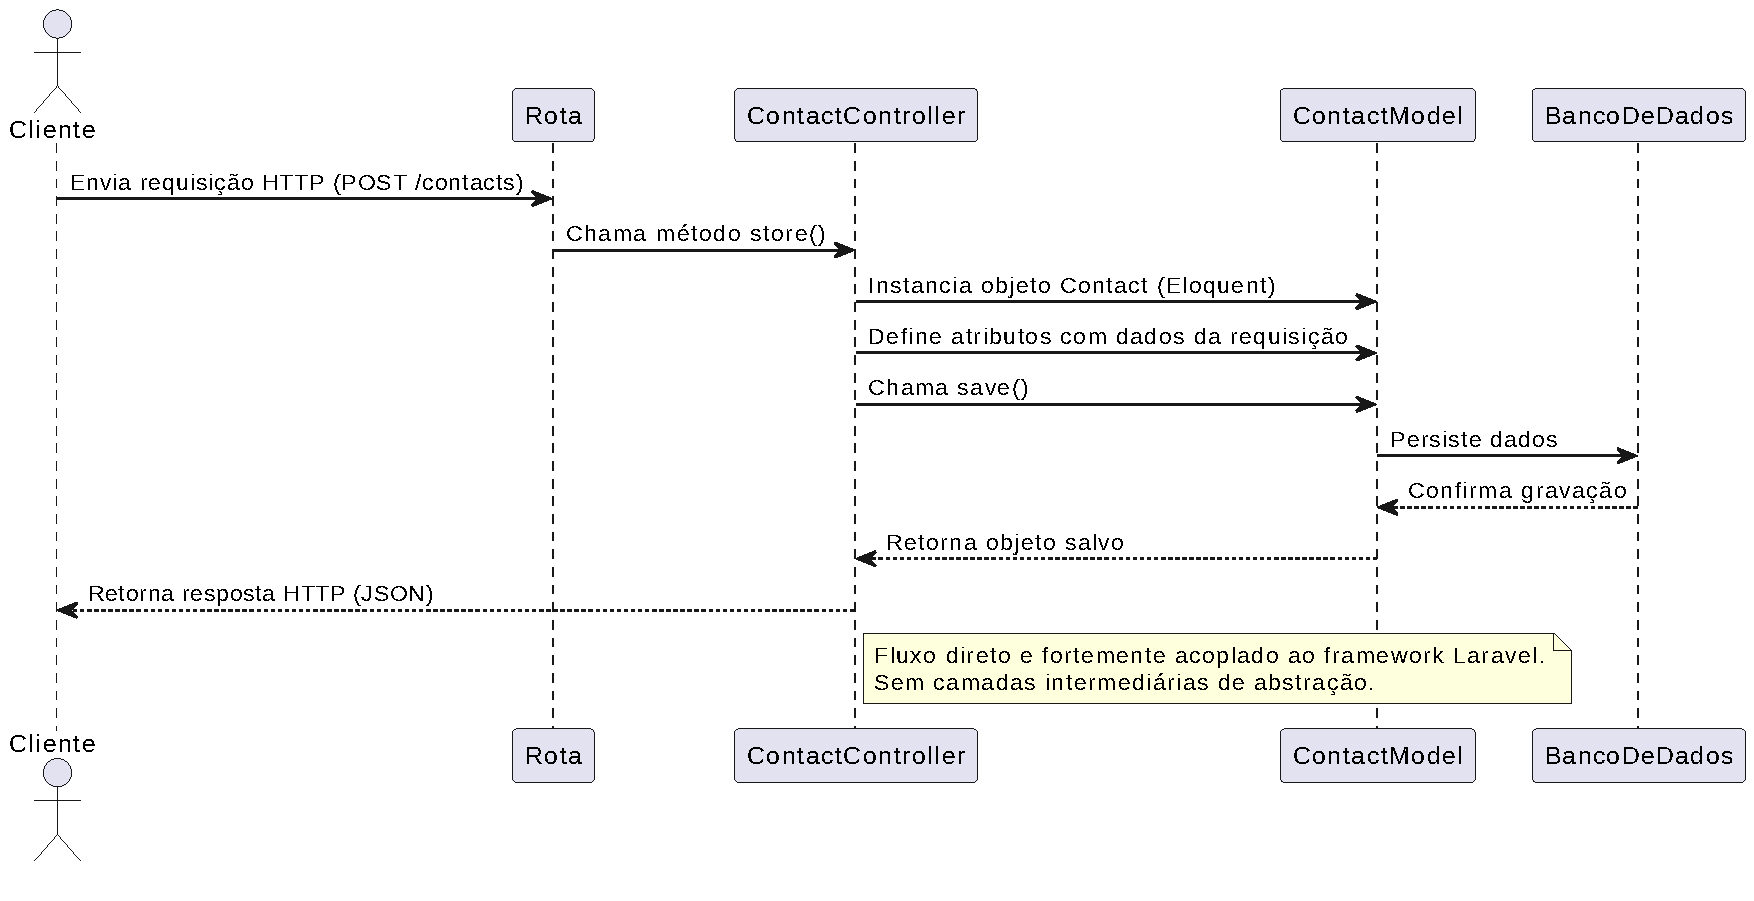
\includegraphics[angle=-90,width=0.5\linewidth]{figuras/resultados/mvc1.pdf}
            \caption{Fluxo da Requisição - Arquitetura MVC Original (Laravel).}
            \label{fig:mvc1} 
            \newcommand{\minhafonte}{Fonte: Autor.}
            \minhafonte
        \end{figure}


        \par Com a refatoração para a Arquitetura Limpa, esse mesmo fluxo foi transformado, promovendo um desacoplamento significativo e a inversão das dependências, conforme ilustrado na Figura \ref{fig:ca1}. 
        
        \begin{figure}[H]
            \centering   
            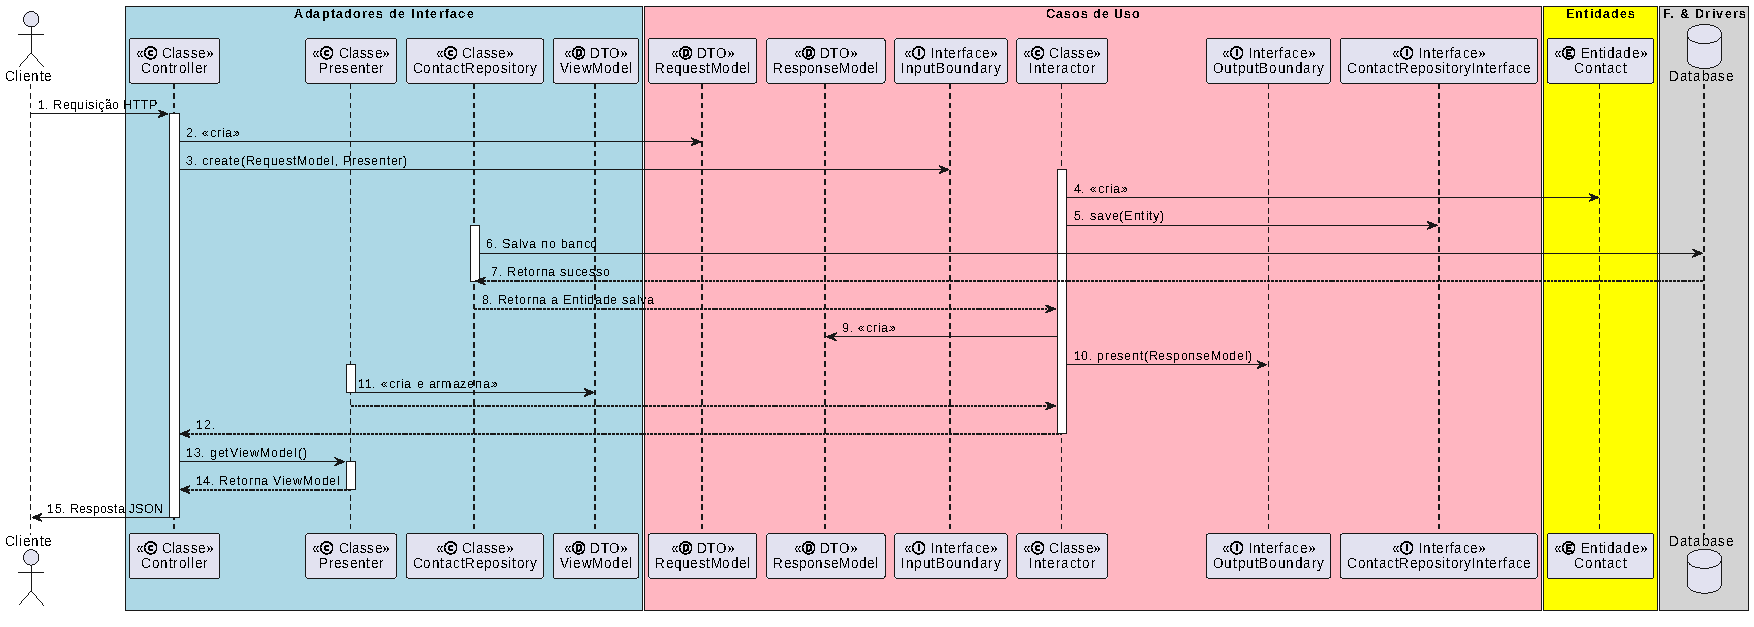
\includegraphics[angle=-90,width=0.5\linewidth]{figuras/resultados/ca1.pdf}
            \caption{Fluxo da Requisição - Arquitetura Limpa (Laravel).}
            \label{fig:ca1}
            \newcommand{\minhafonte}{Fonte: Autor.}
            \minhafonte
        \end{figure}
        
        \par Agora, a requisição HTTP (1) ainda é recebida pelo Controller, que atua como um Adaptador de Interface. Sua primeira ação é criar um RequestModel (2), um DTO que encapsula os dados da requisição de forma agnóstica. Em seguida, o Controller invoca o caso de uso através da sua fronteira, a interface InputBoundary (3), passando o DTO e uma instância do Presenter.

        \par O Interactor, na camada de Casos de Uso, é então ativado e orquestra a lógica de negócio: ele cria a Entidade Contact (4), aplicando as regras de negócio, e delega a persistência para outra abstração, a ContactRepositoryInterface (5). A implementação concreta deste repositório, que também é um Adaptador de Interface, é responsável por interagir com o banco de dados (6, 7, 8). 
        
        \par Ao receber a confirmação da persistência, o Interactor cria um ResponseModel (9) e o envia para a OutputBoundary através do método present() (10), cumprindo sua única responsabilidade. O Presenter, por sua vez, converte os dados em um ViewModel (11). Finalmente, o controle retorna ao Controller, que solicita o ViewModel ao Presenter (13, 14) e envia a resposta JSON final ao cliente (15). Essa abordagem garante que o núcleo da aplicação (Casos de Uso e Entidades) permaneça completamente isolado dos detalhes de infraestrutura, como o framework web e o banco de dados, seguindo estritamente a Regra da Dependência.